\chapter{\ifcpe ทฤษฎีที่เกี่ยวข้อง\else Background Knowledge and Theory\fi}

การทำโครงงานนี้เริ่มต้นจากการที่เราเล็งเห็นปัญหาของตารางสอบปลายภาคของมหาวิทยาลัยเชียงใหม่ 
ซึ่งตารางสอบของนักศึกษาบางคนอาจจะมีตารางเวลาที่ติดกันมากเกินไป ซึ่งผู้จัดทำเห็นว่าปัญหาการจัดตารางสอบปลายภาค
สามารถแปลงเป็นปัญหาที่มีวิธีในการแก้ไขอยู่แล้วได้ ในบทนี้จะกล่าวถึงผลการศึกษาค้นคว้าทฤษฎีที่เกี่ยวข้อง งานวิจัย หรือโครงงาน ที่เคยมีผู้นำเสนอไว้แล้ว
เพื่อช่วยอธิบายถึงสิ่งต่าง ๆ ที่เกี่ยวข้องกับโครงงานนี้เพื่อให้ผู้อ่านเข้าใจเนื้อหาในบทถัด ๆ ไปได้ง่ายยิ่งขึ้น โดยในบทนี้จะมีเนื้อหาต่าง ๆ ได้แก่ Literature review 
ซึ่งจะกล่าวถึงงานวิจัยต่าง ๆ ที่ได้ศึกษามา และส่วนของอัลกอริทึมที่เกี่ยวข้อง ซึ่งจะกล่าวถึงรูปแบบและวิธีการทำงานของอัลกอริทึมต่าง ๆ 
\section{Literature review}
การกำหนดเวลาสอบปลายภาคเพื่อหลีกเลี่ยงปัญหานักศึกษาคนใด ๆ มีเวลาสอบในช่วงเวลาเดียวกันสามารถแปลงปัญหานี้ให้เป็นปัญหา graph coloring~\cite{mcs} ได้ 
โดยที่จุดแต่ละจุดในกราฟเป็นรายวิชาที่เปิดสอนในภาคการศึกษานั้น 
และเส้นที่เชื่อมแต่ละจุดสองจุดในกราฟแสดงถึงการมีนักศึกษาที่ลงทะเบียนเรียนทั้งสองรายวิชา โดยจุดสองจุดใด ๆ ในกราฟที่มีเส้นเชื่อมกันจะถูกกำหนดสีให้ต่างกัน
ซึ่งแสดงถึงวันและเวลาที่จัดสอบปลายภาคในวิชานั้น ๆ โดยจุดที่มีคนละสีก็จะถูกจัดให้สอบคนละช่วงเวลากัน

การแปลงปัญหาการจัดตารางสอบปลายภาคให้เป็นปัญหา graph coloring จะสามารถแก้ปัญหาการจัดตารางสอบแบบพื้นฐานได้เท่านั้น โดยไม่คำนึงถึงข้อจำกัดอย่างอื่น 
ตัวอย่างเช่น ไม่พิจารณาความจุที่นั่งสำหรับการสอบแต่ละช่วงเวลาของนักศึกษา จำนวนอาจารย์ที่คุมสอบแต่ละช่วงเวลา และการกระจายวิชาสอบสำหรับนักศึกษาแต่ละคน เป็นต้น
ถึงแม้จะไม่กำหนดข้อจำกัดใด ๆ ปัญหา graph coloring ก็เป็นปัญหา NP-complete ด้วยตัวมันเองอยู่แล้ว~\cite{alg-design} 
ซึ่งหมายความว่ายังไม่สามารถหาอัลกอริทึมที่ใช้เวลา polynomial-time ในการแก้ไขปัญหาให้ได้ผลลัพธ์ที่เหมาะสมที่สุด 
ทำให้ต้องใช้วิธีอื่นที่ให้ผลลัพธ์ที่ดีในระดับที่ยอมรับได้ แต่สามารถยืนยันได้ว่าจะได้วิธีการที่สามารถแก้ไขปัญหาได้อย่างแน่นอน 
ซึ่งวิธีการนั้นคือ metaheuristic ซึ่งสามารถหาวิธีการแก้ปัญหาที่ดีได้ในระยะเวลาที่เหมาะสม~\cite{meta-for-vertexcolor}
และสามารถกำหนดข้อจำกัดหรือเงื่อนไขอื่นเพิ่มเติมได้ ทำให้สามารถกำหนดขอบเขตของผลลัพธ์ได้ แต่อาจจะไม่ได้วิธีแก้ปัญหาที่ดีที่สุด

อีกวิธีการที่สามารถใช้แก้ไขปัญหาการจัดตารางสอบได้ก็คือการใช้ memetic algorithms (MA) ซึ่งเป็นวิธีการที่นำ local search มาประยุกต์ใช้กับ genetic algorithm 
เพื่อช่วยให้คำตอบของปัญหานั้น converge ช้าลง \cite{pablo-memetic-algo} ซึ่ง Ender {\"O}zcan เคยได้นำวิธีการนี้มาประยุกต์ใช้ในการแก้ปัญหาการจัดตารางสอบ 
โดยได้สร้าง framework สำหรับออกแบบตัวดำเนินการที่ใช้ในการ crossover และ mutation ของ genetic algorithm ด้วย~\cite{fes}
โดยในการทดลองนี้ได้มีการคำนึงถึงนักศึกษา โดยกำหนดข้อจำกัดของตารางสอบที่ได้ให้ไม่มีนักศึกษาที่ต้องสอบติดกันสองวิชาในแต่ละวัน แต่การจัดตารางสอบในแบบของ {\"O}zcan 
นั้นเป็นการจัดตารางสอบของมหาวิทยาลัย Yeditepe โดยแบ่งตารางสอบเป็นของภาควิชาต่าง ๆ และแบ่งย่อยแยกตามสาขาวิชาอีกที วิธีการนี้ไม่สามารถนำมาใช้กับการจัดตารางสอบของมหาวิทยาลัยเชียงใหม่ได้
เนื่องจากมหาวิทยาลัยเชียงใหม่ มีวิชาศึกษาทั่วไปซึ่งเป็นวิชาที่เปิดให้นักศึกษาจากต่างคณะสามารถลงทะเบียนได้ทำให้มีนักศึกษาเป็นจำนวนมากกว่าที่ความจุที่นั่งสอบของคณะนั้นจะรับไหว
ซึ่งทำให้การจัดตารางสอบโดยใช้วิธีนี้นั้นเป็นไปได้ยากเพราะจำนวนนักศึกษาที่เกินความจุที่นั่งสอบนั้นจะละเมิดข้อจำกัดที่กำหนดไว้ 

\iffalse
\section{Tools}
\subsection{Gurobi Optimizer}
Gurobi Optimizer เป็น Solver ที่ใช้สำหรับแก้ปัญหา optimization โดยที่จะเน้นไปทางด้านของปัญหาต่าง ๆ ดังนี้ 
\begin{itemize}
  \item Linear programming (LP)
  \item Mixed-integer linear programming (MILP)
  \item Quadratic programming (QP)
  \item Mixed-integer quadratic programming (MIQP)
  \item Quadratically-constrained programming (QCP)
  \item Mixed-integer quadratically-constrained programming (MIQCP)
\end{itemize}
ผลลัพธ์ที่ได้จาก Gurobi Optimizer อาจนำมาใช้เป็นตัวเปรียบเทียบประสิทธิภาพกับผลลัพธ์การทำงานที่ได้จากอัลกอริทึมของเรา
\fi
\section{หลักการ แนวคิด และทฤษฏีที่เกี่ยวข้องในการทำโครงงาน }
\subsection{Metaheuristics}
Meta­heuristics~\cite{metaheuris} เป็นวิธีการแก้ไขปัญหาที่ใช้งานกันโดยทั่วไป ซึ่งเป็นวิธีการที่สามารถหาผลลัพธ์ของ optimization problems ได้ดีและเหมาะสมกับเวลาที่ใช้ในการประมวลผล
โดยวิธีเหล่านี้นั้นส่วนใหญ่จะเป็นวิธีการที่มีแรงบันดาลใจมาจากการเรียนแบบหลักการของธรรมชาติและนำมาดัดแปลงเป็นอัลกอริทึมเพื่อใช้ในการแก้ปัญหาต่าง ๆ ตัวอย่างของ metaheuristic algorithms เช่น genetic algorithm, evolutionary computation, simulated annealing, tabu search เป็นต้น
\subsection{Genetic algorithms}
Genetic algorithms เป็นหนึ่งใน metaheuristics ซึ่งเป็นเทคนิคสำหรับค้นหาผลลัพธ์หรือคำตอบโดยประมาณของปัญหา โดยอาศัยหลักการจากทฤษฎีวิวัฒนาการทางชีววิทยาและหลักการคัดเลือกตามธรรมชาติ 
\linebreak กล่าวคือ สิ่งมีชีวิตที่เหมาะสมที่สุดจึงจะอยู่รอด \cite{ga} โดยกระบวนการคัดเลือกได้เปลี่ยนแปลงสิ่งมีชีวิตให้เหมาะสมยิ่งขึ้นด้วยตัวดำเนินการทางพันธุกรรม เช่น การสืบพันธุ์ การแลกเปลี่ยนยีน การกลายพันธุ์ เป็นต้น โดยขั้นตอนการทำงานของ genetic algorithm มีดังนี้ 
\begin{enumerate}
  \item initial population เป็นขั้นตอนเริ่มต้นของอัลกอริทึมซึ่งจะทำการกำหนดชุดข้อมูลผลลัพธ์ เรียกชุดข้อมูลนี้ว่า population ซึ่งชุดข้อมูลนี้จะประกอบไปด้วยผลลัพธ์ที่ถูกเข้ารหัสในรูปแบบของสายอักขระที่แต่ละอักขระเป็นบิต 0 หรือ 1 เรียกแต่ละบิตนี้ว่า gene
  โดยที่แต่ละสายอักขระที่ประกอบจาก genes นี้เรียกว่า chromosome โดยชุดข้อมูลนี้อาจจะสุ่มแต่ละ gene ขึ้นมาเป็นค่าเริ่มต้น
  \item fitness function เป็น function สำหรับใช้ในการคัดเลือกชุดข้อมูลที่เหมาะสมให้สามารถอยู่ต่อไปได้ โดยจะมีการคำนวณค่า fitness scores ให้กับแต่ละ chromosome
  โดย fitness scores จะขึ้นอยู่กับความพอใจในผลลัพธ์ที่ได้ของผู้พัฒนา
  \item genetic operator คือวิธีการในการปรับเปลี่ยนรูปแบบโครงสร้างของ chromosome ที่เหมาะสมสำหรับรุ่นถัดไปของกระบวนการ ซึ่งมีวิธีการอยู่ 3 แบบหลัก ๆ ได้แก่
  \begin{itemize}
  \item selection เป็นการเลือกคู่ chromosome ของข้อมูลที่เหมาะสม เพื่อให้ chromosome คู่นี้ส่งต่อ gene ที่ดีแล้วไปยัง chromosome รุ่นถัดไป โดยจะเลือก chromosome ที่มีค่า fitness scores มากที่สุด
  \item crossover เป็นการสุ่มเลือกตำแหน่งระหว่าง genes จาก parent chromosome 1 คู่ โดย genes ด้านซ้ายหรือขวาของจุดแบ่งจะถูกสับเปลี่ยนกันระหว่าง parent chromosome คู่นั้น
  \item mutation เป็นการสุ่มกลับค่าของ gene ใน chromosome ให้มีค่าตรงกันข้ามโดยมีค่าความน่าจะเป็นที่จะเกิด mutation ต่ำ ๆ เพื่อป้องกันไม่ให้ผลลัพธ์ converge ก่อนที่ควรจะเป็น
\end{itemize}
\end{enumerate}
Genetic algorithms สามารถจบการทำงานได้หลายวิธี โดยมีเงื่อนไขในการจบการทำงานดังนี้
\begin{itemize}
  \item จบการทำงานเมื่อ population เปลี่ยนผ่านไปถึงรุ่นที่ต้องการแล้ว 
  \item จบการทำงานหาก population ไม่มีการพัฒนาแล้ว หรือไม่มีการเปลี่ยนแปลงไปในทางที่ดีขึ้นเป็นระยะเวลาหนึ่ง
  \item จบการทำงานเมื่อ fitness scores ของ population มีค่าเท่าที่ต้องการแล้ว
\end{itemize}
\subsection{Graph coloring}
 
Graph coloring เป็นปัญหาที่ได้รับความสนใจอย่างมากในเรื่องทฤษฎีกราฟซึ่งเป็นปัญหาที่เกี่ยวกับการพยายามระบายสีจุดของกราฟ โดยให้จุดที่อยู่ติดกันมีสีต่างกันและใช้สีให้น้อยที่สุด
การระบายสีกราฟอาจมีหลายรูปแบบ บางรูปสามารถใช้สีเพียงสองสีก็เพียงพอที่จะให้จุดที่อยู่ติดกันมีสีต่างกัน บางรูปจำเป็นต้องใช้หลายสีถึงจะเพียงพอที่จะให้จุดที่อยู่ติดกันมีสีต่างกัน 
ดังนั้นจะเรียกจำนวนสีอย่างน้อยที่สุดที่เพียงพอที่จะให้จุดที่อยู่ติดกันมีสีต่างกันว่า จำนวนสีของกราฟ ซึ่งวิธีการระบายสีกราฟมักจะถูกนำไปประยุกต์ใช้กับการแก้ปัญหาการกำหนดตารางเวลา (scheduling problem) 
\subsection{Breadth first search}
Breadth-first search คือ เป็นขั้นตอนการหาข้อมูลทั้งหมดภายในกราฟ โดยเริ่มที่โหนดเริ่มต้นของกราฟ (root) และทำการสำรวจโหนดที่ติดกัน (adjacent node) ไปทีละโหนด โดยสำรวจลงไปทีละระดับของโครงสร้างกราฟ โดยเริ่มจากระดับที่แรก root แล้วลงมาระดับที่ 1 จากซ้ายไปขวา เมื่อเสร็จระดับที่ 1 จะค่อยไปสำรวจที่ระดับที่ 2 จากซ้ายไปขวาเช่นกัน ทําเช่นนี้เรื่อย ๆ
จนพบโหนดที่ต้องการ หรือจนครบทุกโหนด โดยมีลําดับการเดินทางของโหนดเป็นไปตามหมายเลขที่กํากับไว้บนโหนด
ดังรูปที่ \ref{fig:graph_bfs}
\begin{figure}
  \begin{center}
    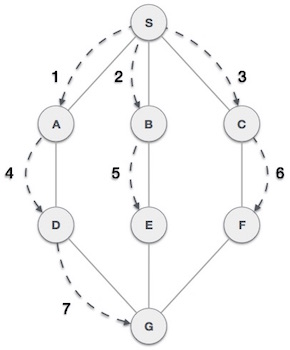
\includegraphics[width=0.5\textwidth]{images/breadth_first_traversal.jpg}
  \end{center}
  \caption[ตัวอย่างการทำ BFS บนกราฟ]{ตัวอย่างการทำ BFS บนกราฟ}
  \label{fig:graph_bfs}     
\end{figure}
\section{\ifcpe%
ความรู้ตามหลักสูตรซึ่งถูกนำมาใช้หรือบูรณาการในโครงงาน
\else%
ISNE knowledge used, applied, or integrated in this project
\fi
}
\begin{itemize}
  \item 261218 Algorithms for Computer Engineers ได้นำวิธีดำเนินงาน หลักการและทฤษฏี ดังนี้มาใช้เพื่อแก้ไขปัญหาในโครงงานนี้  
  \begin{itemize}
  \item วิธีการคิดและวิเคราะห์ปัญหา
  \item วิธีการแปลงปัญหาใหญ่ที่แก้ไขยากให้กลายเป็นปัญหาย่อยที่เล็กกว่าเพื่อใช้วิธีการที่มีอยู่แล้วในการแก้ไขปัญหาย่อยนั้นและนำไปสู่การแก้ปัญหาใหญ่ได้สำเร็จ
  \item ทฤษฏี Graph coloring
  \item การแก้ปัญหา Scheduling problem
  \item การแก้ปัญหา NP-complete และ NP-hard
  \end{itemize}
\end{itemize}

\section{\ifcpe%
ความรู้นอกหลักสูตรซึ่งถูกนำมาใช้หรือบูรณาการในโครงงาน
\else%
Extracurricular knowledge used, applied, or integrated in this project
\fi
}
ความรู้นอกหลักสูตรที่ใช้สำหรับการแก้ไขปัญหาของโครงงานเพื่อให้ได้ผลลัพธ์ที่เหมาะสุดที่สุด เราได้ทำการศึกษา หลักการและทฤษฏี ดังนี้
\begin{itemize}
  \item Meta­heuristics
  \item Genetic algorithms
  \item การสร้างเว็ปแอพพลิเคชันด้วย Vue.js, Node.js, Express
  \item การใช้งาน Database MongoDB
\end{itemize}
